\documentclass[10pt,pdf,hyperref={unicode}]{beamer}

% \documentclass[aspectratio=43]{beamer}
% \documentclass[aspectratio=1610]{beamer}
% \documentclass[aspectratio=169]{beamer}

\usepackage{lmodern}
\usepackage[russian]{babel}

% подключаем кириллицу 
%\usepackage[T2A]{fontenc}
\usepackage[T1]{fontenc}
\usepackage[utf8]{inputenc}
\usepackage{bm}

% отключить клавиши навигации
\setbeamertemplate{navigation symbols}{}

% тема оформления
\usetheme{Madrid}

% цветовая схема
\usecolortheme{whale}

\title[UDE]{Универсальные дифференциальные уравнения}   
\subtitle{Комбинация лучших сторон разных подходов.}
\author{Влад Темкин} 



\institute[HSE] % (optional)
{
	Высшая Школа Экономики\\
	Факультет Физики
}

\date[\today]
{Стохастические процессы и моделирование}

\AtBeginSection[]
{
	\begin{frame}
		\frametitle{План доклада}
		\framesubtitle{Основные моменты}
		\tableofcontents[currentsection]
	\end{frame}
}

\begin{document}
	
	\begin{frame}
		\titlepage
	\end{frame} 
	
	
	\begin{frame}
		\frametitle{План доклада} 
		\framesubtitle{Основные моменты}
		\tableofcontents[pausesections]
	\end{frame}


	\section{Подходы к описанию мира}
	
		\subsection{Физические модели}
		
			\begin{frame}
				\frametitle{Подходы к описанию мира} 
				\framesubtitle{Физические модели}
					\begin{columns}
						\column{0.5\linewidth}
						\begin{center}
							\begin{itemize}
								\item хорошо интерполируют (очень хорошо)
								\item легко интерпретировать 
								\item указывают на структуру процесса
								\item нужно понимать хоть что-то о мире
								\item проигрывают другим моделям (а именно машинному обучению), когда речь идёт о предсказаниях просто из набора данных
							\end{itemize}
						\end{center}
						\column{0.5\linewidth}
							\begin{displaymath}
								\frac{d}{dt}\frac{\partial L}{\partial \dot{x}} - \frac{\partial L}{\partial x} = 0
							\end{displaymath}
							\newline
							\begin{displaymath}
								\left\{\begin{gathered}
									\nabla \cdot \vec{D} = 4\pi	\rho\\
									\nabla \cdot \vec{B} = 0 \\
									\nabla \times \vec{E} = \frac{1}{c}\frac{\partial \vec{B}}{\partial t} \\
									\nabla \times \vec{H} = \frac{4\pi}{c}\vec{j} + \frac{1}{c}\frac{\partial \vec{D}}{\partial t}
								\end{gathered}\right.
							\end{displaymath}
					\end{columns}
			\end{frame}
		
		
		\subsection{Машинное обучение}
		
			\begin{frame}
				\frametitle{Подходы к описанию мира} 
				\framesubtitle{Машинное обучение}
					\begin{columns}
						\column{0.5\linewidth}
							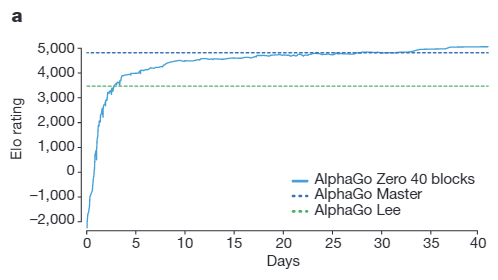
\includegraphics[width=\linewidth]{alphago.png}
							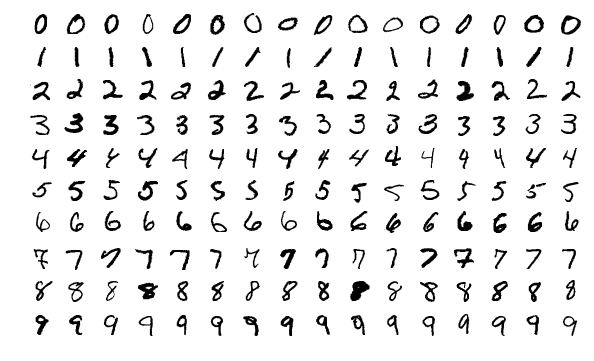
\includegraphics[width=\linewidth]{mnist.png}
						\column{0.5\linewidth}
						\begin{center}
							\begin{itemize}
								\item может решить почти любую задачу
								\item превосходит человека во многих областях
								\item потенциал кажется безграничным (обучение с подкреплением)
								\item сложно интерпретировать
								\item не всегда хорошо интерполирует  
								\item требуется много данных
							\end{itemize}
						\end{center}
					\end{columns}
			\end{frame}
			
			
	\section{Комбинирование двух подходов}
		
		\begin{frame}
			\frametitle{Комбинирование двух подходов} 
			\framesubtitle{Различные практики}
				\begin{block}{Универсальная теорема аппроксимации}
					Нейронная сеть может аппроксимировать любую непрерывную функцию $R^n \to R^m$ с любой заданной точностью.
				\end{block}  
		\end{frame}
		
		
	\section{Универсальные дифференциальные уравнения}
	
		\begin{frame}
			\frametitle{Универсальные дифференциальные уравнения} 
			\framesubtitle{Выделенный случай}
				диффур, заменяем слагаемое на нейронку 
		\end{frame}
	
	
	\section{Вспомогательные инструменты}
	
		\subsection{алгортим SINDy}
		
			\begin{frame}
				\frametitle{Вспомогательные инструменты} 
				\framesubtitle{Алгоритм SINDy}
					тут пару слов о том как робит синди  
			\end{frame}
		
		
	\section{Примеры применения UDE}
	
		\begin{frame}
			\frametitle{Примеры применения UDE} 
				задачи бывают всякие разные  
		\end{frame}
	
		
		\subsection{Модифицированная модель SEIR}
		
			\begin{frame}
				\frametitle{Примеры применения UDE} 
				\framesubtitle{Модифицированная модель SEIR}
					история о том как я код пиздил  
			\end{frame}
			
			
		\subsection{Модель Лотки-Вольтерра}
			
			\begin{frame}
				\frametitle{Примеры применения UDE} 
				\framesubtitle{Модель Лотки-Вольтерра}
					история о том как я код пиздил  во второй раз
			\end{frame}
		
		
	\section*{Литература}
	
		\begin{frame}
			\frametitle{Список литературы} 
				\begin{itemize}
					\item
				\end{itemize}
			
		\end{frame}

\end{document}